%%%%%%%%%%%%%%%%%%%%%%%%%%%%%%%%%%%%%%%%%
% Wenneker Assignment
% LaTeX Template
% Version 2.0 (12/1/2019)
%
% This template originates from:
% http://www.LaTeXTemplates.com
%
% Authors:
% Vel (vel@LaTeXTemplates.com)
% Frits Wenneker
%
% License:
% CC BY-NC-SA 3.0 (http://creativecommons.org/licenses/by-nc-sa/3.0/)
% 
%%%%%%%%%%%%%%%%%%%%%%%%%%%%%%%%%%%%%%%%%

%----------------------------------------------------------------------------------------
%	PACKAGES AND OTHER DOCUMENT CONFIGURATIONS
%----------------------------------------------------------------------------------------

\documentclass[11pt]{scrartcl} % Font size

%%%%%%%%%%%%%%%%%%%%%%%%%%%%%%%%%%%%%%%%%
% Wenneker Assignment
% Structure Specification File
% Version 2.0 (12/1/2019)
%
% This template originates from:
% http://www.LaTeXTemplates.com
%
% Authors:
% Vel (vel@LaTeXTemplates.com)
% Frits Wenneker
%
% License:
% CC BY-NC-SA 3.0 (http://creativecommons.org/licenses/by-nc-sa/3.0/)
% 
%%%%%%%%%%%%%%%%%%%%%%%%%%%%%%%%%%%%%%%%%

%----------------------------------------------------------------------------------------
%	PACKAGES AND OTHER DOCUMENT CONFIGURATIONS
%----------------------------------------------------------------------------------------

\usepackage{amsmath, amsfonts, amsthm} % Math packages

\usepackage{listings} % Code listings, with syntax highlighting

\usepackage[english]{babel} % English language hyphenation

\usepackage{graphicx} % Required for inserting images

\usepackage{booktabs} % Required for better horizontal rules in tables

\numberwithin{equation}{section} % Number equations within sections (i.e. 1.1, 1.2, 2.1, 2.2 instead of 1, 2, 3, 4)
\numberwithin{figure}{section} % Number figures within sections (i.e. 1.1, 1.2, 2.1, 2.2 instead of 1, 2, 3, 4)
\numberwithin{table}{section} % Number tables within sections (i.e. 1.1, 1.2, 2.1, 2.2 instead of 1, 2, 3, 4)

\setlength\parindent{0pt} % Removes all indentation from paragraphs

\usepackage{enumitem} % Required for list customisation
\setlist{noitemsep} % No spacing between list items

%----------------------------------------------------------------------------------------
%	DOCUMENT MARGINS
%----------------------------------------------------------------------------------------

\usepackage{geometry} % Required for adjusting page dimensions and margins

\geometry{
	paper=a4paper, % Paper size, change to letterpaper for US letter size
	top=2.5cm, % Top margin
	bottom=3cm, % Bottom margin
	left=3cm, % Left margin
	right=3cm, % Right margin
	headheight=0.75cm, % Header height
	footskip=1.5cm, % Space from the bottom margin to the baseline of the footer
	headsep=0.75cm, % Space from the top margin to the baseline of the header
	%showframe, % Uncomment to show how the type block is set on the page
}

\usepackage[backend=biber,style=ieee,natbib=true]{biblatex} % Use the bibtex backend with the authoryear citation style (which resembles APA)

\addbibresource{bibliography.bib} % The filename of the bibliography

\usepackage[autostyle=true]{csquotes}
%----------------------------------------------------------------------------------------
%	FONTS
%----------------------------------------------------------------------------------------

\usepackage[utf8]{inputenc} % Required for inputting international characters
\usepackage[T1]{fontenc} % Use 8-bit encoding

%\usepackage{fourier} % Use the Adobe Utopia font for the document

%----------------------------------------------------------------------------------------
%	SECTION TITLES
%----------------------------------------------------------------------------------------

\usepackage{sectsty} % Allows customising section commands

\sectionfont{\vspace{6pt}\centering\normalfont\scshape} % \section{} styling
\subsectionfont{\normalfont\bfseries} % \subsection{} styling
\subsubsectionfont{\normalfont\itshape} % \subsubsection{} styling
\paragraphfont{\normalfont\scshape} % \paragraph{} styling

%----------------------------------------------------------------------------------------
%	HEADERS AND FOOTERS
%----------------------------------------------------------------------------------------

\usepackage{scrlayer-scrpage} % Required for customising headers and footers

\ohead*{} % Right header
\ihead*{} % Left header
\chead*{} % Centre header

\ofoot*{} % Right footer
\ifoot*{} % Left footer
\cfoot*{\pagemark} % Centre footer
 % Include the file specifying the document structure and custom commands

%----------------------------------------------------------------------------------------
%	TITLE SECTION
%----------------------------------------------------------------------------------------

\title{	
	\normalfont\normalsize
	\textsc{University of Basel, Departement of Physics}\\ % Your university, school and/or department name(s)
	\vspace{25pt} % Whitespace
	\rule{\linewidth}{0.5pt}\\ % Thin top horizontal rule
	\vspace{20pt} % Whitespace
	{\huge Funnel hopping Monte Carlo: An efficient
method to overcome broken ergodicity \cite{Finkler2020}}\\ % The assignment title
	\vspace{12pt} % Whitespace
	\rule{\linewidth}{2pt}\\ % Thick bottom horizontal rule
	\vspace{12pt} % Whitespace
}

\author{\LARGE Matthias Vogler} % Your name

\date{\normalsize\today} % Today's date (\today) or a custom date

\begin{document}

\maketitle % Print the title

%----------------------------------------------------------------------------------------
%	FIGURE EXAMPLE
%----------------------------------------------------------------------------------------

\section{Markov Chain Monte Carlo}
The goal of Markov chain Monte Carlo (MCMC) is to generate samples of a target distribution. In our case the target distribution will always be the Boltzmann distribution
\begin{equation}
	P(\mathbf{r})=\frac{1}{Z(t)}\exp\left(\frac{-E(\mathbf{r})}{k_B T}\right)
\end{equation}
We start with a initial configuration $\mathbf{r}$, we then propose a new configuration $\mathbf{r}'$ and accept the new configuration with probability $\alpha$ given by the Metropolis-Hastings criterion \cite{Hastings1970}
\begin{equation}
	\alpha=\text{min}\left(1,\frac{P(\mathbf{r}')}{P(\mathbf{r})}\frac{g(r|r')}{g(r'|r)}\right),
	\label{metropolis}
\end{equation}
where $P(\mathbf{r})$ is our target distribution and $g(r|r')$ the probability to propose a move from $r$ to $r'$. The heart of MCMC lies in proposing the right moves. The displacements should be sufficently small or the moves will always be rejected and a convergent solution will not be found. On the other hand, proposing moves that are too small will result again in almost no progress. Thus there is a inherent trade of between the proposed moves and the acceptance rate. Another problem that arises in MCMC when trying to sample a configuration space to calculate a quantity of a system (e.g. heat capacity) are high energy barriers between different regions of minima, especially at low temperatures of interest. This leads to never sampling the whole configuration space and to the namesake phenomenon of broken ergodicity which the paper of \citeauthor{Finkler2020} tries to overcome with their novel method of \emph{Funnel Hopping Monte Carlo}.\\
\subsection{Energy landscapes and Funnels}
Energy landscapes can best be characterized by their local minima. These minima can be grouped into together with the higher lying minima into so-called \emph{funnels}. Different funnels are usaly seperated by high energy barriers which can't be overcome in the computation time available. This concept is best visualized with energy disconnectivity graphs as seen in figure \ref{fig:funnels}.

\begin{figure}[h!]
	\center
	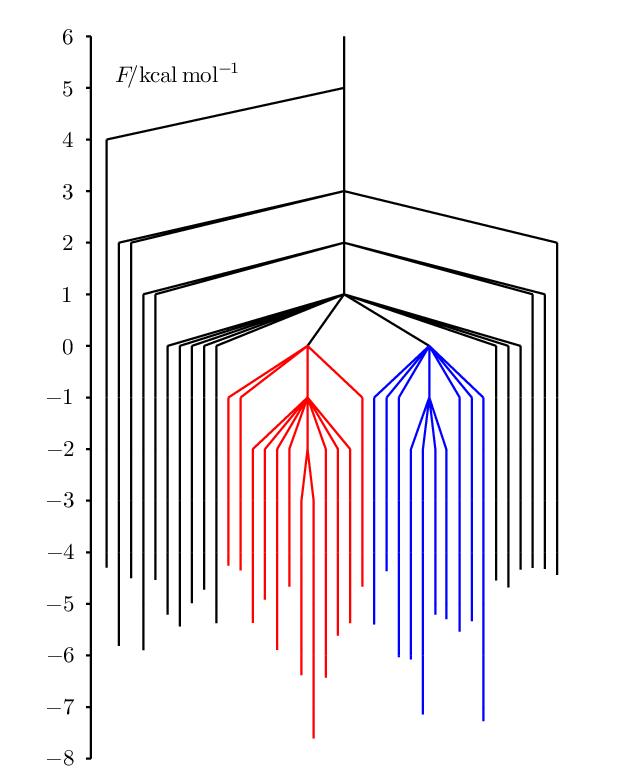
\includegraphics[scale=0.3]{figures/funnels.png}
	\label{fig:funnels}
	\caption{Energy disconnectivity graph for met-enkephalin at 298 K. The low-energy region of the graph contains two funnels, highlighted in red and blue. Source: \cite{Wales2005}}
\end{figure}
\subsection{Already available methods: Paralell Tempering}
Paralell Tempering (PT) is a MC method that runs many copies of the system in paralell at different temperatures. The idea is then to make configurations at high temperatures available to the simulations at low temperatures. This is useful since at high temperatures it is much more likely to overcome higher energy barriers. This information is the passed down to the low temperature instances. The method however has the drawback of being computationaly expensive since many instances have to be run in paralell.

\section{Funnel Hopping Monte Carlo}
The basic idea of Funnel Hopping Monte Carlo (FHMC) is to use precomputed knowledge about the local minima in the energy landscape. This includes the location of the minima which can easily be extracted with global optimization methods such as minima hopping. To construct the FHMC method, there are a lot of preliminary steps one has to take. This will be explained in the following sections.
\subsection{Smart darting}
The main idea of smart darting \cite{Andricioaei2001} is to construct special moves out of the knowledge of the minima. Given a set of $M$ local minima $\{\mathbf{R}_i\}_{i=1,2,\ldots,M}$, we can define \emph{darting vectors} $\mathbf{D}_{ij}$ as 
\begin{equation}
	\mathbf{D}_{ij}=\mathbf{R}_j-\mathbf{R}_i.
\end{equation}
Arround each minima epsilon regions are placed. Configurations can now lie within a minima with the criterion
\begin{equation}
	||\mathbf{R}_i-\mathbf{r}_i||<\epsilon
\end{equation}
with $\epsilon$ chosen such that the regions don't overlap. We can then replace a certain fraction of the MC moves with darting moves. If a darting move is to be executed, first we check if the current configuration $\mathbf{r}$ lies within a $\epsilon$ region of a minima $\mathbf{R}_i$. If true, a darting vector starting at $i$ will randomly be chosen and a new configuration is proposed with
\begin{equation}
	\mathbf{r}'=\mathbf{r}+\mathbf{D}_{ij}
\end{equation}
and accepted or rejected with the standard Metropolis criterion (eq. \ref{metropolis}). This method works very well in some cases. But it has some key problems in certain systems. If we have systems with invariances such as rotation and translations as in clusters, the epsilon regions become hard to define. The minima don't correspond to a single point in configuration space, but rather a hypersurface. This is further exacerbated in systems with indistinguishable atoms which are invariant under permutations. It then becomes impossible to to define these regions with the method described earlier. It also assumes spherical epsilon regions, where as in reality regions of low energy are often ellipsoidal. It is therefore important to have a method which makes no assumptions about the shape of the high probability regions.
\subsection{Removing degrees of freedom: Eckart space}
To decide if a configuration is inside the high probability regions, we have to be able identify similar configurations. In 3$N$ dimensional configuration space it is non trivial to identify similar configurations which are rotaionally invariant. To do this, we first select a reference configuration $\mathbf{R}$ in a local minima. We then try to identify the optimal rotaion $\mathcal{R}$ and permutation $\mathcal{P}$ of $\mathbf{r}$ such that the root mean squared deviation (RMSD) is minimal. We define the RMSD as
\begin{equation}
	\text{RMSD}(\mathbf{r},\mathbf{R})=\sqrt{\frac{\sum_{i=1}^N ||\vec{r_i}-\vec{R}_i||}{N}}
\end{equation}
We define the displacement $\mathbf{d}$ as
\begin{equation}
	\vec{d}_i=\vec{r}_i-\vec{R}_i.
\end{equation}
The RMSD is then minimal if the modified \emph{Eckart conditions} are met \cite{Kudin2005}:
\begin{equation}
	\sum_{i=1}^N \vec{d}_i= \vec{0}
	\label{eq:1}
\end{equation}
\begin{equation}
	\sum_{i=1}^N \vec{d}_i\times \vec{R}_i = \vec{0}
	\label{eq:2}
\end{equation}
We can now define vectors, to which all displacement vectors obtained with minimal RMSD alignement are orthogonal to:
\begin{equation}
	V^1=\begin{pmatrix} 1\\0\\0\\1\\0\\0\\1\\ \vdots\end{pmatrix},
	V^2=\begin{pmatrix} 0\\1\\0\\0\\1\\0\\0\\ \vdots\end{pmatrix},
	V^3=\begin{pmatrix} 0\\0\\1\\0\\0\\1\\0\\ \vdots\end{pmatrix},
	V^4=\begin{pmatrix}0 \\ \vec{R}_{1,z} \\ -\vec{R}_{1,y} \\ 0 \\ \vec{R}_{2,z} \\ -\vec{R}_{2,y} \\ 0 \\ \vdots \end{pmatrix},
	V^5=\begin{pmatrix}-\vec{R}_{1,z} \\ 0 \\ \vec{R}_{1,x} \\ -\vec{R}_{2,z} \\ 0 \\ \vec{R}_{2,x} \\ \vec{R}_{3,z} \\ \vdots\end{pmatrix},
	V^6=\begin{pmatrix}\vec{R}_{1,y}\\-\vec{R}_{1,x}\\0\\\vec{R}_{2,y}\\-\vec{R}_{2,x}\\0\\\vec{R}_{3,y}\\\vdots\end{pmatrix}
\end{equation}
This gives as the possibility to construct $3N-6$ new basis vectors $B^i$ that are orthogonal to the vectors $V^j$. Using $B^i$ as our new basis removes 6 degrees of freedom from our system and fixes rotation and translation. The $3N$ dimensional vector $\mathcal{d}$ is then transformed via
\begin{equation}
	\mathbf{d}'=\mathbf{d}\cdot\mathbf{B}^i
\end{equation}
To get the total minimum of the RMSD in systems of indistinguishable atoms, one has to minimize with respect to permutations as well. There however, one encounters a causality dilemma. The optimal rotation depends on the permutation where as the optimal permutation depends on the optimal rotation. The paper however suggests a clever method using the Hungarian algorithm \cite{Kuhn1955} in conjunction with a quaternion method \cite{Coutsias2004}.
\subsection{Funnel Hopping Monte Carlo}
With the procedures described above, we can finaly get to the actual method at hand. First we assign each point in configuration space to its nearest minimum. For each minimum $\mathbf{R}_i$ one defines a probability distribution $q_i(\mathbf{r})$ which lives in the $3N-6$ dimensional fixed frame corrdinate space. To propose a Funnel Hopping move one determines the nearest minimum $\mathbf{R}_i$ to the current configuration and randomly chooses another minimum $j$. Then one draws a configuration from the corresponding $q_j$. Determining $j$ can be done completly random or via a transition matrix $T$ with $T_ij$ being the probability to choose $j$ while being in minimum $i$. This can help with proposing moves that connect minima with similar energy. The move is then accepted or rejected over a modified Metropolis criterion:

\begin{equation}
	\alpha(\mathbf{r}\rightarrow\mathbf{r}')=\text{min}\left(1,\exp\left(-\frac{E(\mathbf{r}')-E(\mathbf{r})}{k_BT}\right)\frac{q_i(\mathbf{r})}{q_j(\mathbf{r}')}\frac{T_{ji}}{T_{ij}}\frac{h_{\alpha i}}{h_{\alpha j}}\right)	
\end{equation}
The distributions $q_i$ are still undefined, but they main role they play is that they are used to generate the proposed configuration. The paper proposes to define these distributions over gaussian mixtures which are defined as follows:
\begin{equation}
	q_i^{g.m.}(r)=\left.\sum_{k=1}^m a_i^k \mathcal{N}_i^k(r) \quad\right|\quad \sum_{k=1}^m a_i^k=1\text{ and } a_i^k \geq0\,\forall k
\end{equation}
with $\mathcal{N}_i^k$ are normalized multivariate Gaussians with means $\mu^k_i$ and covariance $\Sigma_i^k$. The parameters $a_i^k$, $\mu_i^k$ and $\Sigma_i^k$ are then fitted to the Boltzmann distribution.


\newpage
\printbibliography[heading=bibintoc]
\end{document}
